\section{Theorie}
\label{sec:Theorie}
\subsection{Brechung von Licht}
\label{subsec:brechung}
Durchdringt ein Lichtstrahl die Grenzfläche zweier Medien, in denen die Ausbreitungsgeschwindigkeiten
des Lichtes unterschiedlich sind, so wird er gebrochen. Dies wird durch das Snellius'sche
Brechungsgesetz beschrieben:
\begin{equation}
  n=\frac{v_1}{v_2}=\frac{\sin(\alpha)}{\sin{\beta}} \,.
  \label{eqn:snelluis}
\end{equation}
Dabei sind $v_{\symup{i}}$ die Lichtgeschwindigkeiten im jeweiligen Medium. $\alpha$
und $\beta$ geben den Winkel an, den die Strahlen vor und nach der Brechnug mit der
Normalen der Grenzfläche einschließen. Eine Skizze hierzu ist in Abbildung \ref{fig:brechung}
zu sehen.

\begin{figure}[H]
  \centering
  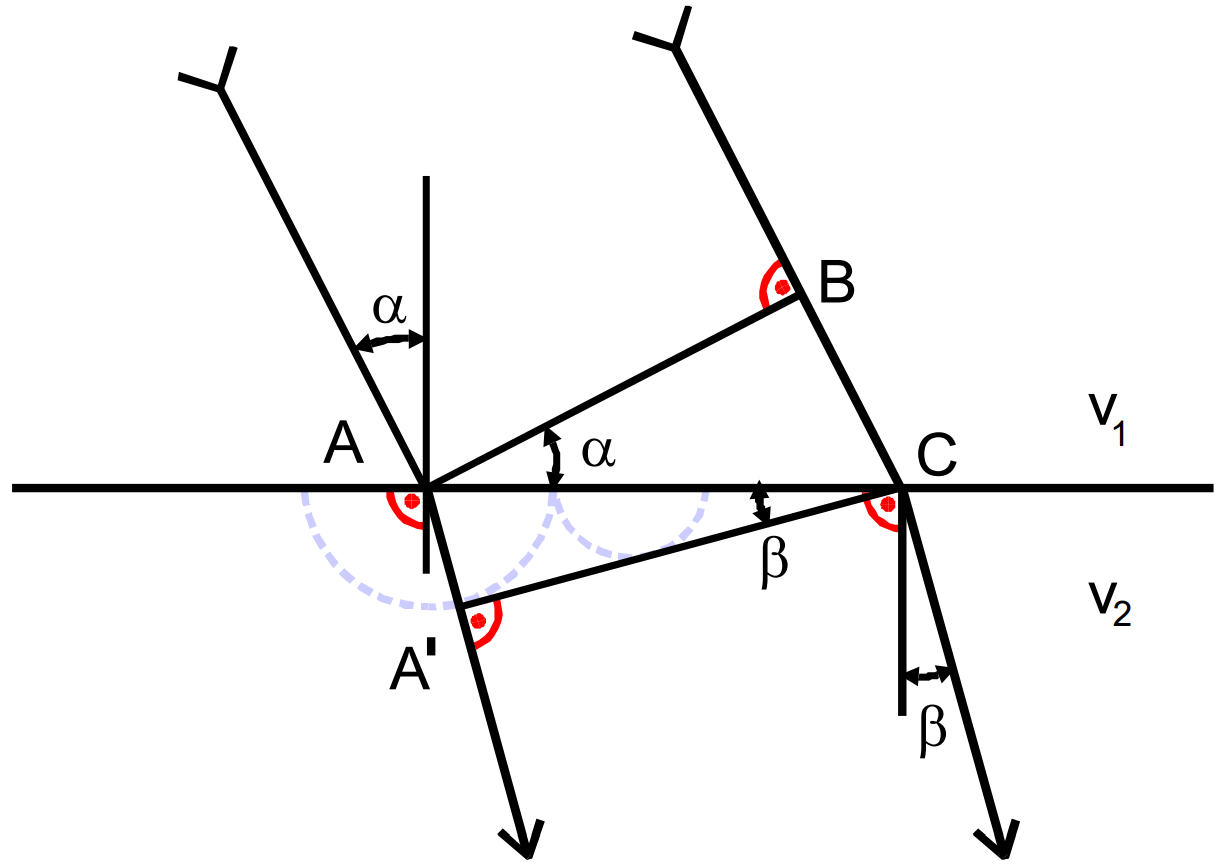
\includegraphics[height=5cm]{data/brechung.png}
  \caption{Brechung von Lichtstrahlen an einer Grenzfläche \cite{Versuchsanleitung}.}
  \label{fig:brechnung}
\end{figure}

Das Snellius'sche Brechungsgesetz kann auch aus dem Huygens'schen Prinzip der Elementarwellen
hergeleitet werden.

\subsection{Herleitung der Dispersion}
\label{subsec:dispersion1}
Der Begriff Dispersion beschreibt einen Zusammenhang zwischen Brechungsindex $n$ und
Wellenlänge $\lambda$. Wird der Brechungsindex mit sinkender Wellenlänge des Lichts
größer, so liegt normale Dispersion vor. Der umgekehrte Fall wird anormale Dispersion
genannt.

Unter einigen Annahmen lässt sich für einen Festkörper eine Dispersionsgleichung
herleiten. Es muss dabei beachtet werden, dass die lokalisierten, elektrisch geladenen
Bestandteile des Festkörpers berücksichtigt werden. Diese befinden sich in Gleichgewichtslagen,
die durch Licht angeregt werden können. Für bestimmte Wellenlängen treten dabei
Resonanzen auf. Bei diesen Wellenlängen absorbiert der Festkörper einen großen Teil
des Lichts. Im Folgenden sollen nur Bereiche betrachtet werden, für die keine
Absorption auftritt.

Um eine Gleichung für die Bewegung der Teilchen im Festkörper zu erhalten, wird
angenommen, dass diese von einer ebenen Lichtwelle angeregt und durch eine Reibungskraft,
die proportional zur Teilchengeschwindigkeit ist, abgebremst werden. Es ergibt sich
die Differentialgleichung
\begin{equation}
  m_{\symup{h}}\frac{\symup{d}^2\,\symbf{x_{\symup{h}}}}{\symup{d}\,t^2}
  +f_{\symup{h}}\frac{\symup{d}\,\symbf{x_{\symup{h}}}}{\symup{d}\,t}
  +a_{\symup{h}}\symbf{x_{\symup{h}}}=q_{\symup{h}}\symbf{E_0}\exp(i \omega t)\,.
  \label{eqn:diff}
\end{equation}
Dabei ist $m_{\symup{h}}$ die Teilchenmasse,$f_{\symup{h}}$ der Reibungskoeffizient
bei der Bewegung der Teilchen, $a_{\symup{h}}$ die Beschleunigung (???) der Teilchen,
$q_{\symup{h}}$ die Ladung der Teilchen, $\symbf{E_0}$ das elektrische Feld der Lichtwelle,
$\omega$ deren Frequenz, $t$ die Zeit.

\subsection{Näherungen der Dispersionskurve}
\label{subsec:dispersion2}

Aus Gleichung \eqref{eqn:diff} kann ein Zusammenhang zwischen der Wellenlänge $\lambda$ des
Lichts und dem komplexen Brechnugsindex $\tilde{n}$ hergeleitet werden:
\begin{equation}
  \tilde{n}^2=1+\sum_{\symup{h}}\frac{1}{\omega_{\symup{h}}^2-\omega^2
  +i\frac{f_{\symup{h}}}{m_{\symup{h}}}\omega} \frac{N_{\symup{q}} q_{\symup{h}}^2}
  {m_{\symup{h}} \epsilon_0} \,.
\end{equation}
Dabei ist $\omega_{\symup{h}}^2$ die Resonanzfrequenz und $N_{\symup{h}}$ die
Teilchenanzahl pro Volumeneinheit. Zwischen $\tilde{n}$ und $n$ gilt der Zusammenhang
\begin{equation}
  \tilde{n}=n(1-ik)\,,
\end{equation}
wobei $k$ die Absorptionskonstante des Lichts in Materie ist. Wie zuvor bereits erwähnt,
soll hier nicht weiter auf die Absorption eingegangen werden, sodass
\begin{equation}
  n^2k\approx0
\end{equation}
gelten soll. Damit ergibt sich die der Zusammenhang
\begin{equation}
  {n}^2 (\lambda) = \symbf{1}+\sum_{\symup{h}} \frac{N_{\symup{h}}q_{\symup{h}}^2}
  {4 \pi^2 c^2 \epsilon_0 m_{\symup{h}}}
  \frac{\lambda^2 \lambda_{\symup{h}}^2}{\lambda^2-\lambda_{\symup{h}}^2}
  \label{eqn:dispersion}
\end{equation}
zwischen Brechungsindex $n$ und Wellenlänge $\lambda$.

Nun wird der Fall betrachtet, dass der Festkörper eine Absorptionsstelle
$\lambda_{\symup{a}}$ beseitzt. Dann lassen sich grundsätzlich die beiden Fälle
$\lambda \gg \lambda_{\symup{a}}$ und $\lambda \ll \lambda_{\symup{a}}$ unterscheiden.
Für den ersten Fall lässt sich Gleichung \eqref{eqn:dispersion} nach Potenzen von
$\lambda_{\symup{a}}/\lambda$ entwickeln. Dann ergibt sich
\begin{equation}
  n^2(\lambda)=A_0+\frac{A_2}{\lambda^2}+\frac{A_4}{\lambda^4}+... \,.
  \label{fall1}
\end{equation}
Dabei müssen die $A_{\symup{i}}$ größer als Null sein.

Für den zweiten Fall lässt sich Gleichung \eqref{eqn:dispersion} zu
\begin{equation}
  n^2(\lambda)=1-A_2'\lambda^2-A_4'\lambda^4-...
  \label{fall2}
\end{equation}
entwickeln. Hier müssen die $A_{\symup{i}}'$ für $i≥2$ größer als Null sein.

In Abbildung \ref{fig:faelle} sind die Dispersionskurven für beide Fälle skizziert.
Es ist erkennbar, dass der Brechungsindex mit steigender Wellenlänge sinkt. Beide
Formeln beschreiben also normale Dispersion.

\begin{figure}[H]
  \centering
  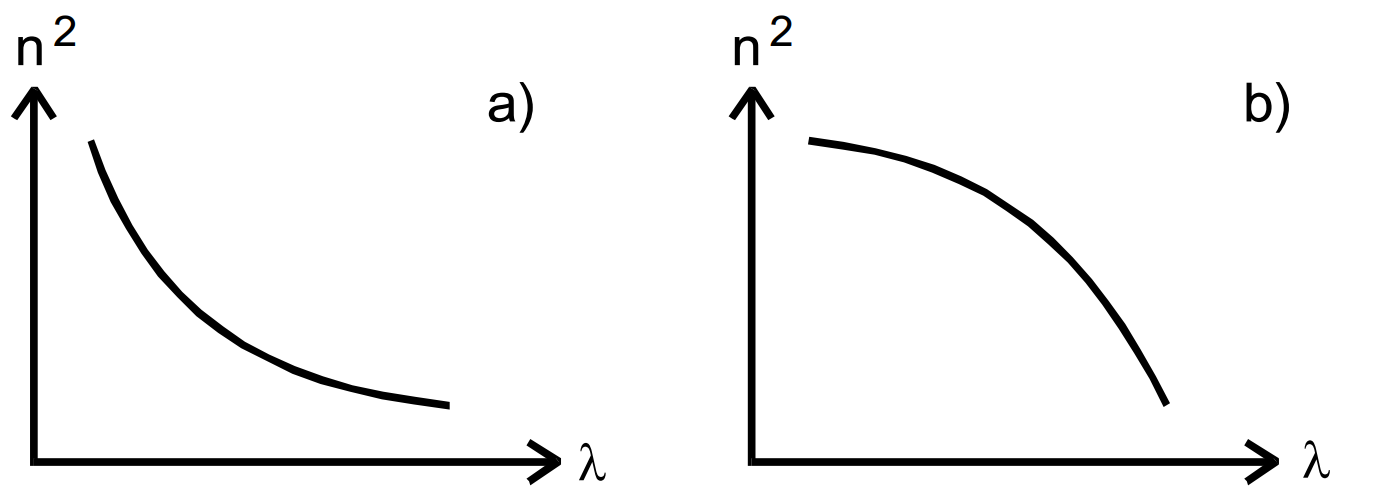
\includegraphics[height=5cm]{data/dispersionskurve.png}
  \caption{Skizze der Dispersionskurven der beiden Fälle \cite{Versuchsanleitung}.}
  \label{fig:faelle}
\end{figure}

\subsection{Grundlagen für die Messung und deren Auswertung}
\label{subsec:messung}

Im Versuch sind Winkel die Winkel $\eta$ und $\phi$ zu bestimmen, aus denen sich
der Brechungsindex gemäß
\begin{equation}
  n=\frac{\sin\left(\frac{\eta+\phi}{2}\right)}{\sin\left(\frac{\phi}{2}\right)}
  \label{eqn:n_aus_winkeln}
\end{equation}
berechnen lässt.

Außerdem soll später die Abbe'sche Zahl
\begin{equation}
  \nu=\frac{n_{\symup{D}}-1}{n_{\symup{F}}-n_{\symup{C}}}
\end{equation}
berechnet werden. Diese ist ein Maß für die Dispersion des Materials.
Die $n_{\symup{i}}$ bedeuten dabei die Brechungsindices des
verwendeten Materials für die Fraunhofer'schen Linien mit $\lambda_{\symup{C}}=656\,$nm,
$\lambda_{\symup{D}}=589\,$nm und $\lambda_{\symup{F}}=486\,$nm.

Zudem soll das Auflösungsvermögen untersucht werden. Dieses ist definiert durch
\begin{equation}
  A=\frac{\lambda}{\Delta\lambda} \,.
\end{equation}
Es kann gezeigt werden, dass gilt:
\begin{equation}
  \frac{\lambda}{\Delta\lambda}=b\frac{\symup{d}\,n}{\symup{d}\,\lambda} \,.
\end{equation}
Dabei ist $n$ der Brechungsindex und $b$ die Seitenlänge des verwendeten Prismas.
